\chapter{Estudios complementarios de rescate de ensamble}\label{app:complementarios}

Este anexo conserva el estudio de ensambles y poda desarrollado durante el proyecto. Su rescate contiene varios clasificadores sobre subconjuntos y no equivale a ejecutar la misma concatenación Top-k del cuerpo principal. Sus resultados OOF, presupuestos y réplicas no se atribuyen automáticamente a la comparación directa/por margen de esta tesis. Se preservan como evidencia complementaria, incluidos los casos desfavorables y las reservas de costo proyectado.


\section{Bloques, miembros y política de adquisición}
Sea $\mathcal B=\{1,\ldots,M\}$ una biblioteca de extractores congelados. El bloque $j$ transforma una imagen $x_i$ en $\mathbf z_{ij}\in\mathbb R^{d_j}$. Para un subconjunto $S\subseteq\mathcal B$, se utiliza
\begin{equation}
\mathbf z_{i,S}=\mathop{\Vert}_{j\in S}
\frac{\mathbf z_{ij}}{\max(\lVert\mathbf z_{ij}\rVert_2,10^{-12})},
\qquad d_S=\sum_{j\in S}d_j .
\label{eq:concat}
\end{equation}
Cada miembro $f_S$ es una SVM entrenada sobre una concatenación de bloques; distintos votos pueden corresponder al mismo modelo. Una política $\pi=(b,E,\tau)$ consta de un bloque base $b$, una lista de miembros de rescate $E$ y un umbral $\tau$. El ensamble completo puede contener miembros repetidos con efecto en el voto, aunque cada modelo único se ejecute una sola vez.

La biblioteca comprende 22 bloques y 20.652 dimensiones nominales. Los descriptores fijos se almacenan por imagen, mientras que la proyección SVD de N-gramas se aprende con el entrenamiento del ajuste pertinente. Los detalles de extracción, checkpoints y dimensiones se conservan en el Anexo~\ref{app:especificaciones}. La selección actúa sobre bloques completos, no sobre coordenadas individuales.

Se denomina entrenamiento productor al conjunto utilizado para construir candidatos, seleccionar la política y reajustar los modelos. Dentro de él se obtienen predicciones OOF internas para la selección. La validación productora permanece fuera de esas decisiones y evalúa la política elegida. El Capítulo~\ref{sec:diseno} detalla ambos niveles de partición.

\section{Generación del ensamble de subconjuntos}
Se construye un ensamble de 15 miembros, cada uno con cuatro bloques. La relevancia $R_j$ se obtiene normalizando $a_j$, la media aritmética del macro-F1 individual entre los pliegues internos:
\begin{equation}
R_j=\frac{a_j-a_{\min}}{a_{\max}-a_{\min}},
\label{eq:relevance}
\end{equation}
con denominador uno cuando todos los valores coinciden. La frontera de bases y las ganancias de poda, en cambio, usan macro-F1 sobre las predicciones OOF internas reunidas. Ambas agregaciones pueden producir ordenamientos diferentes. La similitud entre dos matrices de características centradas por columna, $X$ e $Y$, se calcula mediante CKA lineal \citep{kornblith2019similarity}:
\begin{equation}
\operatorname{CKA}(X,Y)=
\frac{\lVert Y^\top X\rVert_F^2}
{\lVert X^\top X\rVert_F\,\lVert Y^\top Y\rVert_F}.
\label{eq:cka}
\end{equation}
Si el denominador es cero, la implementación devuelve cero. Se usa únicamente el entrenamiento productor, es decir, las imágenes disponibles para construir y seleccionar la ruta antes de evaluar su pliegue de validación.

Dado el conjunto parcial $S$, la utilidad de un candidato es
\begin{equation}
u_j(S)=R_j-\lambda\,|S|^{-1}\sum_{\ell\in S}\operatorname{CKA}(j,\ell);
\qquad u_j(\varnothing)=R_j .
\label{eq:utility}
\end{equation}
Los candidatos se ordenan por utilidad decreciente y nombre en caso de empate. Si quedan $n$ candidatos y $r_j=1$ identifica el mejor, el sorteo utiliza
\begin{equation}
p(j\mid S)=\frac{(n-r_j+1)^\beta}{\sum_{\ell=1}^{n}\ell^\beta}.
\label{eq:lottery}
\end{equation}
Cada bloque elegido se retira del sorteo del mismo miembro. Entre miembros sí pueden repetirse subconjuntos. En el piloto se fijaron $\beta=8$ y $\lambda=0{,}25$, procedentes de la configuración archivada del ensamble. No se presentan como hiperparámetros óptimos universales.

\section{Puntuaciones y agregación}
Cada SVM produce un vector de puntuaciones $s_S(x)\in\mathbb R^C$, con el mismo orden de clases. Su escala $\sigma_S$ es la desviación estándar poblacional de todas las puntuaciones de sus imágenes de entrenamiento, agrupando filas y clases. Se fija en uno si no es positiva o finita. La puntuación normalizada es
\begin{equation}
\widetilde s_S(x)=s_S(x)/\sigma_S,\qquad
\widehat y_E(x)=\arg\max_c\frac{1}{|E|}
\sum_{S\in E}\widetilde s_{S,c}(x).
\label{eq:ensemble}
\end{equation}
La escala permanece congelada en validación; no se recalcula con el lote evaluado. Esta operación no convierte las puntuaciones en probabilidades calibradas. Los miembros repetidos conservan su multiplicidad en la suma del ensamble completo. El rescate podado, en cambio, usa pesos uniformes sobre modelos únicos seleccionados.

\section{Base y compuerta}
Las bases candidatas pertenecen a la frontera no dominada de macro-F1 individual interno y costo proyectado. Una base se excluye si otra no es peor en calidad ni costo y la mejora estrictamente en al menos uno. Es una restricción del espacio de búsqueda: no demuestra que una base dominada individualmente carezca de utilidad para enrutamiento.

El margen de la base es la diferencia entre sus dos puntuaciones más altas:
\begin{equation}
m_b(x)=\widetilde s_{b,(1)}(x)-\widetilde s_{b,(2)}(x).
\label{eq:margin}
\end{equation}
Para cada base se consideran cuantiles $q\in\{0{,}1;0{,}25;0{,}5\}$ de márgenes OOF internos. Un umbral $\tau_{b,q}$ define la regla
\begin{equation}
\widehat y_\pi(x)=
\begin{cases}
\widehat y_b(x),& E=\varnothing\ \text{o}\ m_b(x)\ge\tau_{b,q},\\
\widehat y_E(x),& m_b(x)<\tau_{b,q}.
\end{cases}
\label{eq:decision-rule}
\end{equation}
Cuando se activa el rescate, su predicción reemplaza a la base; esta no se añade como voto adicional. El margen ordena las muestras para esta regla de parada, pero no es una probabilidad de acierto. Tras reajustar la base con todo el entrenamiento productor, su escala se vuelve a estimar únicamente con ese entrenamiento y se conserva el valor numérico del umbral OOF. No se recalcula el cuantil con la validación productora. Por ello, el cuantil seleccionado no fija una fracción exacta de derivación al evaluar.

\section{Costo compartido y presupuesto}
Sea $U(E)$ la unión de bloques de los miembros y $c_j$ el costo por extractor del perfil fijado. Para la fracción interna derivada $\widehat r$, se estima
\begin{equation}
\widehat C(b,E)=
\begin{cases}
c_b,&E=\varnothing,\\
c_b+c_{\mathrm{pol}}+\widehat r
\displaystyle\sum_{j\in U(E)\setminus\{b\}}c_j,&E\ne\varnothing.
\end{cases}
\label{eq:cost-hybrid}
\end{equation}
Los bloques compartidos se contabilizan una vez y la representación base se reutiliza. El piloto fija $c_{\mathrm{pol}}=0{,}45$ ms como sobrecosto del perfil. Este valor no constituye un cronometraje de todos los clasificadores del híbrido. El Anexo~\ref{app:especificaciones} registra las constantes utilizadas.

Los presupuestos $B\in\{15,30,60,120\}$ ms restringen la media proyectada de selección, no el costo de cada imagen ni una media futura. La fracción derivada puede cambiar al evaluar. También se registra el número esperado de llamadas:
\begin{equation}
\widehat L=1+\widehat r\,|\operatorname{unique}(E)|.
\end{equation}
Menos llamadas no implica por sí solo una reducción física proporcional.

\subsection{Interpretación del costo de adquisición}
Para una política no vacía, sea $A_{b,E}=\sum_{j\in U(E)\setminus\{b\}}c_j$ el costo adicional del rescate. El modelo por imagen es
\begin{equation}
C_\pi(x)=c_b+c_{\mathrm{pol}}+
\mathbb I[m_b(x)<\tau]\,A_{b,E}.
\end{equation}
La media de esta expresión da la Ecuación~\ref{eq:cost-hybrid}. El sobrecosto fijo se aplica a todas las imágenes cuando existe rescate, no solo a las derivadas.

Una referencia que extrae permanentemente la misma unión tiene costo de adquisición $C_E=\sum_{j\in U(E)}c_j$, sin incluir latencia de clasificadores. Si $A_{b,E}>0$, la política condicional reduce ese costo estimado únicamente cuando
\begin{equation}
\widehat r < \frac{C_E-c_b-c_{\mathrm{pol}}}{A_{b,E}}.
\label{eq:break-even}
\end{equation}
La condición muestra dos efectos distintos: podar puede reducir $U(E)$ y enrutar puede reducir $\widehat r$. Una base fuera de la unión añade un costo que debe compensarse; el umbral también puede derivar demasiadas imágenes para que la adquisición resulte ventajosa. Esta identidad del modelo de costos no es una garantía de latencia física. Además, comparar un rescate podado condicional con un ensamble completo permanente cambia ambos mecanismos, por lo que no aísla el aporte de la compuerta.

\section{Selección completa y poda del rescate}
Sea $\mathcal P_B$ la familia restringida de políticas visitadas a partir de las bases candidatas, los cuantiles y la búsqueda de rescates para el presupuesto $B$. Se selecciona
\begin{equation}
\widehat\pi_B\in
\underset{\pi\in\mathcal P_B:\,\widehat C(\pi)\le B}
{\operatorname{arg\,max}}\;
\widehat F_{1,\mathrm{OOF}}(\pi),
\label{eq:policy-selection}
\end{equation}
donde el macro-F1 se calcula sobre las puntuaciones internas reunidas. El desempate favorece menor costo, menos miembros y, finalmente, los identificadores deterministas de la implementación. La optimalidad se refiere solo a los puntos visitados en $\mathcal P_B$; no a todos los subconjuntos posibles. Si ninguna base cabe en el presupuesto, la configuración se registra como inviable.

El criterio operativo de este estudio es maximizar calidad interna dentro de un presupuesto de adquisición fijado, no aceptar una pérdida de F1 elegida después de observar validación. Al evaluar se informan conjuntamente $\Delta F_1$, costo y cumplimiento del presupuesto frente a controles factibles para el mismo $B$. Una política domina descriptivamente a otra si no empeora ninguna de las dos magnitudes y mejora al menos una; de otro modo se conserva el compromiso, sin agregarlo en una puntuación arbitraria. No se escoge un presupuesto de despliegue ni se establece un margen retrospectivo de no inferioridad. Una excedencia en validación se registra como incumplimiento observado, aunque la selección interna fuera factible.

El rescate completo compara la base sola con los 15 votos para cada base, cuantil y presupuesto factibles. La poda empieza sin miembros y añade hasta tres modelos únicos del mismo ensamble. Cada adición debe mejorar el macro-F1 interno de la ruta y cumplir $\widehat C\le B$. Se comparan dos méritos:
\begin{equation}
h_{\mathrm{rel}}=\Delta F_1,\qquad
h_{\mathrm{marg}}=\Delta F_1/\Delta\widehat C .
\end{equation}
Aquí $\Delta F_1$ es el cambio de macro-F1 de la ruta completa sobre las imágenes internas reunidas, manteniendo base y umbral; no el F1 aislado del candidato ni el F1 de las imágenes derivadas solamente. $\Delta\widehat C$ es la diferencia de costo de adquisición al añadir ese miembro a los ya elegidos.
El primer criterio se denomina \emph{relevancia} en los registros, pero su mérito es la ganancia de macro-F1 de la ruta, no la relevancia individual $R_j$ usada para generar el ensamble. Solo se aceptan ganancias mayores que $10^{-12}$. En el criterio marginal, una ganancia positiva con costo incremental no mayor que $10^{-12}$ tiene prioridad sobre razones finitas; el criterio de relevancia ordena por ganancia sin utilizar ese cociente. Los desempates consideran ganancia, costo y nombre del miembro. Se conserva el mejor punto interno visitado, incluida base sola.

Esta es una búsqueda heurística sobre candidatos generados, no una solución global del problema combinatorio. La relevancia y la razón marginal usan el mismo pool, bases y cuantiles; cambiar ese pool constituiría otra comparación.

\begin{table}[H]
\centering
\caption{Procedimiento de selección dentro de un entrenamiento productor. La validación productora no interviene en estos pasos.}
\label{tab:algoritmo-entrenamiento}
\begin{minipage}{0.95\textwidth}\small
\begin{enumerate}
\item Recibir entrenamiento productor, biblioteca, grupos, semilla y perfil de costos.
\item Calcular ranking individual y CKA; generar 15 subconjuntos de cuatro bloques.
\item Obtener puntuaciones OOF internas de bases y miembros, ajustando SVD y escalas dentro de cada ajuste pertinente.
\item Construir la frontera de bases; para cada presupuesto y cuantil, evaluar base sola y rescate completo o la secuencia de poda.
\item Conservar la política de mayor macro-F1 interno bajo el presupuesto y los desempates especificados.
\item Reajustar los modelos necesarios con el entrenamiento productor; congelar escalas y umbral. Guardar selección e índices antes de evaluar la validación productora.
\end{enumerate}
\end{minipage}
\end{table}

\begin{table}[H]
\centering
\caption{Especificación de inferencia de la política seleccionada. El piloto la evalúa sobre puntuaciones guardadas; la ejecución física completa del híbrido no ha sido medida.}
\label{tab:algoritmo-inferencia}
\begin{minipage}{0.95\textwidth}\small
\begin{enumerate}
\item Extraer y normalizar la base; calcular su predicción y margen.
\item Si no hay rescate o el margen es al menos el umbral, devolver la predicción base.
\item En otro caso, adquirir $U(E)\setminus\{b\}$, reutilizando cada bloque ya disponible.
\item Evaluar cada modelo único del rescate; agregar puntuaciones con sus escalas y multiplicidades fijadas. Devolver la clase de mayor puntuación.
\end{enumerate}
\end{minipage}
\end{table}
\FloatBarrier

\begin{figure}[!htbp]
\centering
\begin{tikzpicture}[
  box/.style={draw,rounded corners,align=center,text width=7.0cm,minimum height=1.1cm,inner sep=5pt,font=\fontsize{9}{11}\selectfont},
  smallbox/.style={draw,rounded corners,align=center,text width=4.3cm,minimum height=1.0cm,inner sep=5pt,font=\fontsize{9}{11}\selectfont},
  arr/.style={-{Stealth[length=2mm]},thick}
]
\node[box,fill=blue!6] (train) {Entrenamiento productor\\Ranking, CKA y miembros candidatos};
\node[box,fill=blue!6,below=7mm of train] (select) {OOF interno: seleccionar base, rescate\\y umbral bajo presupuesto};
\node[box,fill=blue!6,below=7mm of select] (freeze) {Reajustar modelos y congelar política\\antes de la validación productora};
\draw[arr] (train) -- (select);
\draw[arr] (select) -- (freeze);
\node[smallbox,fill=green!6,below=9mm of freeze] (base) {Imagen: bloque base\\Predicción y margen};
\node[smallbox,fill=green!6,below left=10mm and 2mm of base] (exit) {Sin rescate o $m\ge\tau$\\Devolver clase base};
\node[smallbox,fill=orange!10,below right=10mm and 2mm of base] (rescue) {$m<\tau$: adquirir unión\\de bloques faltantes};
\node[smallbox,fill=orange!10,below=7mm of rescue] (vote) {Modelos únicos y voto\\Rescate reemplaza base};
\draw[arr,dashed] (freeze) -- (base);
\draw[arr] (base) -- (exit);
\draw[arr] (base) -- (rescue);
\draw[arr] (rescue) -- (vote);
\end{tikzpicture}
\caption{Construcción de la política y especificación de su ejecución. La selección usa entrenamiento; la compuerta utiliza el margen de cada imagen, no su etiqueta. En el piloto las rutas se reconstruyen con puntuaciones guardadas y costos proyectados; no se cronometra esta ruta completa desde RGB.}
\label{fig:hibrido-flujo}
\end{figure}
\FloatBarrier


\section{Referencias estáticas y cascada de comparación}
\label{sec:comparadores}
Las estrategias estáticas son: Individual, mejor descriptor interno; Completa, los 22 bloques; GFS, selección secuencial; Top-$k$, los primeros del ranking individual con $k$ heredado de GFS; y Homogénea, GFS restringido a una familia con el límite de tamaño del GFS heterogéneo. Top-$k$ controla composición bajo igual número de bloques, no una elección independiente de $k$.

GFS inicia vacío y añade el bloque que maximiza macro-F1 interno, hasta ocho bloques. Se detiene tras dos mejoras consecutivas menores que 0,001 y devuelve el mejor paso visitado. Sus detalles y esquema se conservan en el Anexo~\ref{app:especificaciones}.

La cascada de referencia usa una base y una concatenación Top-$k$ archivada como rescate. Su compuerta deriva si $m(x)\le\tau$, mientras el híbrido usa $m(x)<\tau$. El umbral se seleccionó entre cuantiles 0,25/0,50/0,75 minimizando costo bajo tolerancia interna de F1 de 0,005. La ruta Top-$k$ no se reconstruyó dentro de cada pliegue productor OOF; esta dependencia se mantiene como límite de esa referencia. Si ninguna ruta cumple, se elige Top-$k$ directo.

En la referencia se consideraron ResNet-50, SigLIP, BEiT-v2 y ConvNeXt V2; KTH utilizó solo ResNet-50 y BEiT-v2. No se confunde este conjunto acotado de bases con la frontera individual del híbrido.

\section{Piloto de rescate de ensamble}
Sea $D_{\mathrm{dev}}$ el entrenamiento oficial de Outex. Cada pliegue productor $h$ lo divide en entrenamiento $T_h$ y validación $V_h$, sin grupos compartidos. A su vez, $T_h$ se divide en tres pliegues internos. Se distinguen cuatro operaciones:
\begin{enumerate}
\item Construir el ranking, calcular CKA y generar los subconjuntos utilizando $T_h$.
\item Reunir puntuaciones OOF internas de las imágenes de $T_h$ y seleccionar base, umbral y rescate mediante la Ecuación~\ref{eq:policy-selection}.
\item Reajustar los modelos elegidos con $T_h$, estimar sus escalas y conservar el umbral numérico seleccionado.
\item Predecir las imágenes de $V_h$ sin modificar la política a partir de sus etiquetas.
\end{enumerate}
Al reunir las tres validaciones $V_h$ se obtienen las 680 predicciones OOF de desarrollo, una por imagen y política. Esas predicciones son distintas de las puntuaciones OOF internas que guiaron la selección.

La biblioteca de candidatos se construye a nivel de $T_h$; no se genera de nuevo dentro de cada pliegue interno. Las puntuaciones internas, por tanto, sirven como criterio de selección dentro de una búsqueda adaptada a $T_h$, no como evaluación independiente del procedimiento completo. La evaluación productora conserva separadas las imágenes de $V_h$. La semilla de partición productora es 142 y la interna, 42; el Anexo~\ref{app:procedencia} registra tamaños y multiplicidades.

El piloto reutiliza puntuaciones de validación productora de los miembros del control de diversidad previamente auditado. Se ajustaron las puntuaciones internas faltantes y las bases necesarias, comprobando igualdad de particiones y procedencia. Los parámetros del ensamble, presupuestos y cuantiles se fijaron desde la configuración de desarrollo; no son una preespecificación ciega de toda la investigación.

Los controles del mismo piloto incluyen mejor individual interno, Top-3/4/5, Completa-22 y ensamble de diversidad permanente. Top-3/4/5 son tamaños fijos; no equivalen al Top-$k$ del benchmark que hereda $k$ de GFS. Se añadió un ensamble estático seleccionado bajo cada presupuesto, definido a continuación; no se dispone de GFS concatenado reajustado para este protocolo.

\subsection{Ablación del mismo rescate con y sin compuerta}\label{sec:diseno-p0}
Se reconstruyeron cuatro vistas de cada una de las doce políticas a partir de puntuaciones y predicciones de validación productora guardadas: base sola, mismo rescate permanente, ruta forzada y ruta condicional. Se conservaron los miembros, multiplicidades, pesos, escalas, modelos y particiones; no se reentrenó ni se utilizó el test oficial. La base de cada vista es la elegida para esa política, no el mejor individual global.

El rescate permanente predice todas las imágenes con los miembros fijados y contabiliza únicamente la unión $U(E)$, sin extraer una base innecesaria. La ruta forzada conserva además la base y el sobrecosto de política, pero activa el mismo rescate en todas las imágenes. Ambas producen las mismas clases; la segunda tiene otra contabilidad de costo y llamadas. La vista condicional conserva la decisión archivada de la compuerta. Si el rescate es vacío, las cuatro vistas se reducen a la base; esos casos no aportan evidencia sobre enrutamiento.

El contraste entre rescate permanente y condicional aísla la activación para los modelos fijados en este archivo de desarrollo. No evalúa el mejor rescate estático posible: sus miembros fueron seleccionados conjuntamente con la compuerta. Las doce configuraciones reutilizan las mismas 680 imágenes y son dependientes. Se informan cambios predictivos, costos y llamadas, sin atribuirles significancia confirmatoria ni equivalencia poblacional.

\subsection{Control estático bajo presupuesto}\label{sec:diseno-estatico-presupuesto}
En cada entrenamiento productor se reúnen los 22 clasificadores individuales y los modelos únicos del ensamble de diversidad, con las puntuaciones OOF internas guardadas. Se enumeran todos los ensambles de uno a tres miembros únicos de ese pool, con igual peso y sin repetición. Para cada presupuesto 15, 30, 60 y 120 ms se elige el mayor macro-F1 interno cuya unión de bloques sea factible. Los desempates favorecen menor costo, menos modelos y orden léxico. No se añade una base ni una compuerta al costo del control permanente.

Las doce decisiones se guardaron antes de calcular sus predicciones de validación productora. Se reutilizaron nueve modelos disponibles y se reajustaron nueve con la misma receta SVM y el mismo entrenamiento productor. La enumeración es exhaustiva dentro de ese pool y límite de tres miembros, no sobre todas las concatenaciones o ponderaciones posibles. Se conservan los mismos pliegues y constantes del híbrido; el control no sustituye una ejecución GFS bajo presupuesto.

Este análisis se diseñó después de conocer el piloto y P0. Su regla se fijó antes de obtener las nuevas predicciones, pero no constituye una preinscripción ciega. Se conserva todo el barrido y no se usa el test oficial ni se reajusta el híbrido a partir del resultado del control.

\subsection{Réplica en FMD y semillas adicionales}\label{sec:diseno-replica}
La réplica conserva la biblioteca de 22 bloques, SVM, tres pliegues productores y tres internos, presupuestos 15/30/60/120 ms y cuantiles 0,10/0,25/0,50. Mantiene cinco sorteos de candidatos de tamaño cuatro, hasta tres miembros podados y el ensamble de quince votos con $\beta=8$ y $\lambda=0{,}25$. No se modificaron estos parámetros a partir de sus resultados. Las cinco condiciones y los comandos se fijaron antes de ejecutar la cola, después de conocer el piloto; no constituyen una preinscripción ciega de la investigación.

En FMD se reserva el pliegue externo 0 de la partición estratificada y agrupada de cada semilla 42, 123 y 2026: 800 imágenes forman $D_{\mathrm{dev}}$ y las 200 restantes quedan excluidas. En Outex se mantiene el entrenamiento oficial de 680 imágenes y se añaden las semillas 123 y 2026, sin evaluar las 680 imágenes de test. El piloto Outex/42 se conserva por separado. Las semillas alteran particiones, sorteos y transformaciones; no aíslan solamente el efecto de la inicialización. La partición productora usa semilla $s+100$ y la interna, $s$.

Cada condición evalúa referencias individuales, Top-3/4/5, Completa-22, ensambles permanentes, las tres reglas híbridas y el rival estático bajo presupuesto. La vista P0 vuelve a aplicar permanentemente exactamente el rescate seleccionado, sin reoptimizarlo. La cobertura se audita por imagen, grupo y transformación, manteniendo el test externo excluido. El perfil de costos es el mismo del piloto Outex, no una medición nueva de extracción en FMD. Las reglas completas y el detalle por semilla se conservan en el Anexo~\ref{sec:anexo-replica}.

\section{Resultados del rescate de ensamble en desarrollo Outex}\label{sec:resultados-hibrido}

El piloto usa las 680 imágenes del entrenamiento oficial de Outex, semilla 42, tres folds productores y tres internos. El test oficial no fue evaluado. La Tabla~\ref{tab:hybrid-oof} muestra todas sus políticas; no se comparan directamente con el F1 de test de la Tabla~\ref{tab:tm-cascada}.

\begin{table}[!htbp]
\centering\small
\caption{Controles del mismo piloto Outex: macro-F1 OOF sobre 680 imágenes de entrenamiento oficial y costo medio proyectado, no latencia física.}
\label{tab:controles-hibrido}
\begin{tabular}{@{}lrr@{}}
\toprule
Control & Macro-F1 & Costo proyectado ms\\
\midrule
Individual interno & 0,871642 & 177,300\\
Top-3 & 0,882967 & 236,862\\
Top-4 & 0,884244 & 256,272\\
Top-5 & 0,900824 & 288,435\\
Completa-22 & 0,913957 & 1706,420\\
Diversidad15 permanente & 0,914389 & 365,196\\
\bottomrule
\end{tabular}
\end{table}


\begin{figure}[!htbp]
\centering
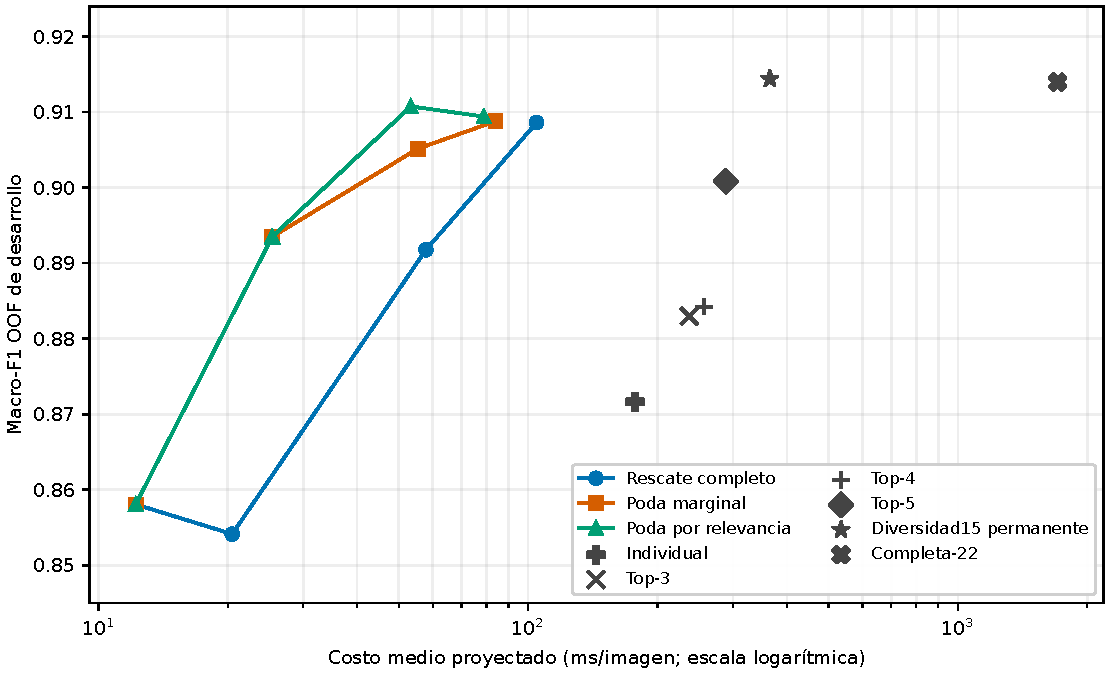
\includegraphics[width=\textwidth]{figures/hibrido_calidad_costo.pdf}
\caption{Políticas del piloto Outex y controles del mismo protocolo. Se muestran los cuatro presupuestos de cada variante, incluidos puntos coincidentes. El eje horizontal es costo proyectado en escala logarítmica, no latencia física; las líneas no representan una frontera óptima.}
\label{fig:hibrido-calidad-costo}
\end{figure}
\FloatBarrier

\begin{table}[!htbp]
\centering\small
\caption{Piloto híbrido de Outex: macro-F1 OOF de desarrollo y costo proyectado. $B$ es el presupuesto de selección en ms; los costos no son latencias físicas.}
\label{tab:hybrid-oof}
\begin{tabular}{@{}lrrr@{}}
\toprule
Ruta & $B$ & Macro-F1 & Costo proyectado ms\\
\midrule
Diversidad15 permanente & -- & 0,914389 & 365,196\\
Completo como rescate & 15 & 0,858056 & 12,220\\
Podado marginal & 15 & 0,858056 & 12,220\\
Podado relevancia & 15 & 0,858056 & 12,220\\
Completo como rescate & 30 & 0,854129 & 20,485\\
Podado marginal & 30 & 0,893488 & 25,394\\
Podado relevancia & 30 & 0,893488 & 25,394\\
Completo como rescate & 60 & 0,891759 & 57,839\\
Podado marginal & 60 & 0,905140 & 55,365\\
Podado relevancia & 60 & 0,910742 & 53,316\\
Completo como rescate & 120 & 0,908603 & 104,660\\
Podado marginal & 120 & 0,908781 & 84,018\\
Podado relevancia & 120 & 0,909396 & 78,938\\
\bottomrule
\end{tabular}
\end{table}

El punto podado por relevancia/B60 obtiene $0{,}910742$, frente a $0{,}914389$ de diversidad permanente, con 85,40\% menos costo estimado y una diferencia de F1 de $-0{,}003646$ (aproximadamente $-0{,}365$ puntos porcentuales). Top-5 obtiene $0{,}900824/288{,}435$ ms y Completa-22 $0{,}913957/1706{,}420$ ms. El híbrido supera numéricamente Top-5, pero no a Completa ni al ensamble permanente en calidad. B60 es un punto observado dentro del barrido de desarrollo, no un presupuesto validado de forma independiente después de su selección.

Ese punto deriva 278/680 imágenes: corrige 52 errores de las bases y perjudica cinco aciertos. El saldo de 47 aciertos adicionales describe exactitud, no una diferencia de macro-F1, que depende de la distribución de errores por clase. Sus bases son DINOv2-small, BEiT-v2-final y VGG16, con dos, dos y un modelos de rescate únicos. Las llamadas medias son 1,654 frente a 10,665 del ensamble permanente. El resto de las imágenes sale por la base; el Anexo~\ref{app:procedencia} aclara la diferencia entre votos y modelos ejecutados.

A presupuesto 15 se elige base sola; el rescate completo/B30 tampoco se activa. Relevancia supera a marginal en calidad y costo en los puntos de 60 y 120 ms. Los 36 presupuestos internos se cumplen, pero completo/B60/fold1 registra 70,019604 ms proyectados en validación frente a 59,602804 internos. Se conservan esa excedencia y la falta de monotonía del F1 con el presupuesto.


La Tabla~\ref{tab:controles-hibrido} y la Figura~\ref{fig:hibrido-calidad-costo} permiten comparar referencias sin trasladar cifras de test externo. El primer control siguiente mantiene fijo el rescate; el segundo lo compara con una selección estática propia bajo presupuesto. GFS concatenado sigue sin evaluarse en este protocolo. El análisis emparejado de N-gramas se conserva como evidencia secundaria en el Anexo~\ref{app:resultados-adicionales}.

\subsection{Separación de poda y activación condicional}\label{sec:resultados-p0}
La Tabla~\ref{tab:p0-b60} descompone el punto relevancia/B60 con el control de la Sección~\ref{sec:diseno-p0}. Son las mismas 680 imágenes y los mismos modelos del piloto; el recálculo no constituye otra evaluación independiente.

\begin{table}[!htbp]
\centering\small
\caption{Control de poda y compuerta en relevancia/B60. Macro-F1 OOF sobre las mismas 680 imágenes; costo medio de adquisición proyectado y llamadas a clasificadores únicos por imagen. No son tiempos físicos.}
\label{tab:p0-b60}
\begin{tabular}{@{}lrrr@{}}
\toprule
Vista & Macro-F1 & Costo ms & Llamadas\\
\midrule
Ensamble completo permanente & 0,914389 & 365,196 & 10,665\\
Mismo rescate podado permanente & 0,911993 & 110,421 & 1,668\\
Mismo rescate, ruta forzada & 0,911993 & 110,871 & 2,668\\
Ruta condicional & 0,910742 & 53,316 & 1,654\\
\bottomrule
\end{tabular}
\end{table}


La poda cambia el ensamble permanente de $0{,}914389/365{,}196$ ms a $0{,}911993/110{,}421$ ms: reduce la adquisición proyectada en 69,76\%, con $\Delta\mathrm{F1}=-0{,}002395$. Activar condicionalmente ese mismo rescate reduce otros 51,72\% respecto de su ejecución permanente, hasta $53{,}316$ ms, con $\Delta\mathrm{F1}=-0{,}001251$. Las reducciones se aplican sucesivamente y no se suman; el descenso total frente al ensamble completo es 85,40\%. La ruta forzada retiene la base y tiene costo $110{,}871$ ms; se distingue de la referencia permanente eficiente, que omite ese trabajo.

Frente al mismo rescate permanente, la compuerta cambia tres clases predichas: corrige una y perjudica dos. La exactitud pasa de $0{,}914706$ a $0{,}913235$. Es un contraste distinto del balance de 52 errores corregidos y cinco aciertos perjudicados frente a las bases. Las llamadas medias apenas disminuyen un 0,79\% respecto del rescate podado permanente, de $1{,}668$ a $1{,}654$. La gran reducción de llamadas frente al ensamble completo corresponde principalmente a la poda, no a la compuerta.

En marginal/B60, las 680 predicciones condicionales coinciden exactamente con las del mismo rescate permanente: macro-F1 $0{,}905140$ y exactitud $0{,}907353$. Su costo proyectado pasa de $97{,}282$ a $55{,}365$ ms, una reducción de 43,09\%. Sin embargo, las llamadas aumentan de $1{,}334$ a $1{,}672$, un 25,36\%, porque la ruta también calcula la base. Menor adquisición proyectada puede coexistir con más evaluaciones de clasificadores; la coincidencia de clases en estas imágenes no prueba equivalencia poblacional.

El barrido completo, incluida la base sola, se presenta en la Tabla~\ref{tab:p0-barrido}. En ocho configuraciones existe rescate: la compuerta reduce F1 en siete y conserva las predicciones en marginal/B60; no mejora F1 en ninguna. Las otras cuatro se reducen a la base. Los rescates permanentes de ambos criterios en B60 superan 60 ms proyectados, mientras sus rutas condicionales quedan por debajo en la media reunida. Esto no descarta una alternativa estática distinta que cumpla el mismo presupuesto. La excedencia del rescate completo/B60 en un pliegue sigue vigente. Para esta ablación no se calcularon valores $p$ ni se midió latencia física.

\subsection{Comparación con selección estática bajo presupuesto}\label{sec:resultados-estatico-presupuesto}
El control de la Sección~\ref{sec:diseno-estatico-presupuesto} cumple su presupuesto en las doce combinaciones de pliegue y presupuesto. Los pools contienen 31, 33 y 34 candidatos. En B60 se examinan 617 combinaciones factibles por pliegue; en B120, entre 1.287 y 1.701. La elección usa únicamente macro-F1 OOF interno. La Tabla~\ref{tab:estatico-presupuesto} conserva los cuatro presupuestos frente a relevancia, sin recomendar uno retrospectivamente.

\begin{table}[!htbp]
\centering\fontsize{8}{10}\selectfont
\caption{Control estático optimizado dentro del pool visitado, con hasta tres miembros, frente al híbrido por relevancia bajo el mismo presupuesto. Macro-F1 OOF de desarrollo sobre 680 imágenes; $C$ es adquisición media proyectada en ms. $\Delta$ es híbrido menos estático.}
\label{tab:estatico-presupuesto}
\begin{tabular}{@{}lrrrrr@{}}
\toprule
$B$ & F1 estático & $C$ estático & F1 híbrido & $C$ híbrido & $\Delta$F1\\
\midrule
15 & 0,859690 & 13,752 & 0,858056 & 12,220 & -0,001634\\
30 & 0,861264 & 28,463 & 0,893488 & 25,394 & 0,032225\\
60 & 0,892923 & 44,831 & 0,910742 & 53,316 & 0,017819\\
120 & 0,909612 & 103,040 & 0,909396 & 78,938 & -0,000216\\
\bottomrule
\end{tabular}
\end{table}


En B30, el híbrido por relevancia tiene mayor F1 observado y menor costo proyectado que el control: $0{,}893488/25{,}394$ ms frente a $0{,}861264/28{,}463$ ms. En B60 obtiene $0{,}910742$ frente a $0{,}892923$, pero también adquiere más información estimada: $53{,}316$ frente a $44{,}831$ ms. Ambos cumplen 60 ms en la media reunida; no son puntos de idéntico costo.

En B15, el estático tiene mayor F1 ($0{,}859690$ frente a $0{,}858056$) y mayor costo ($13{,}752$ frente a $12{,}220$ ms). En B120 también obtiene mayor F1 ($0{,}909612$ frente a $0{,}909396$) con mayor costo ($103{,}040$ frente a $78{,}938$ ms). Por tanto, la comparación no muestra superioridad uniforme de la adquisición condicional. La ventaja predictiva observada dentro de B60 corresponde a este pool, semilla y protocolo de desarrollo; no establece optimalidad global, significancia entre dominios ni aceleración física.
\FloatBarrier

\section{Réplica del rescate en dos datasets}\label{sec:resultados-replica}
Las cinco condiciones nuevas de la Sección~\ref{sec:diseno-replica} completaron sus etapas y la auditoría de índices, selecciones y predicciones. Las medias de la Tabla~\ref{tab:replica-medias} no incluyen el piloto Outex/42: resumen tres semillas FMD y dos semillas Outex. Se conserva relevancia como referencia de la discusión del piloto, sin cambiar la regla para escoger retrospectivamente el mejor resultado de cada fila. Las tres reglas completas y las referencias emparejadas figuran en las Tablas~\ref{tab:replica-barrido} y~\ref{tab:replica-referencias}.

\begin{table}[!htbp]\centering\small
\caption{Réplica de desarrollo: media entre semillas nuevas de macro-F1 / costo proyectado (ms). El número entre paréntesis es el de semillas, no datasets independientes. $B$ restringe el costo interno medio; no es el costo medido. Outex/42 no integra estas medias.}
\label{tab:replica-medias}
\begin{tabular}{@{}lrrr@{}}
\toprule
Dataset & $B$ & Híbrido relevancia & Estático presupuestado\\
\midrule
FMD (3) & 15 & 0,970011 / 11,680 & 0,970011 / 11,680\\
FMD (3) & 30 & 0,974618 / 18,499 & 0,968776 / 14,777\\
FMD (3) & 60 & 0,977489 / 35,689 & 0,974600 / 41,888\\
FMD (3) & 120 & 0,977074 / 46,923 & 0,977082 / 100,929\\
Outex (2) & 15 & 0,862953 / 12,220 & 0,866642 / 13,372\\
Outex (2) & 30 & 0,895551 / 24,224 & 0,874557 / 25,989\\
Outex (2) & 60 & 0,905991 / 40,750 & 0,889152 / 49,047\\
Outex (2) & 120 & 0,908323 / 77,365 & 0,905582 / 109,396\\
\bottomrule
\end{tabular}
\end{table}

\FloatBarrier

En B60, relevancia alcanza en FMD macro-F1 medio $0{,}977489$ y adquisición proyectada $35{,}689$ ms, frente a $0{,}974600/41{,}888$ ms del estático. En las dos semillas nuevas de Outex obtiene $0{,}905991/40{,}750$ ms frente a $0{,}889152/49{,}047$ ms. Son comparaciones bajo un mismo presupuesto de selección, no a idéntico costo realizado ni pruebas de significancia entre dominios. En FMD/B30 el mayor F1 del híbrido requiere más costo; en FMD/B120 las medias de F1 casi coinciden, sin demostrar equivalencia. En Outex/B15 el estático conserva mayor F1 a cambio de mayor adquisición.

El promedio FMD/B60 oculta diferencias importantes entre semillas. En la semilla 42, el estático supera al híbrido en calidad y costo: $0{,}978772/35{,}078$ ms frente a $0{,}977506/38{,}282$ ms. En 123, el híbrido pierde $0{,}000042$ de F1 con menor costo ($35{,}869$ frente a $52{,}565$ ms); en 2026 lo supera en ambas medidas. Tampoco se conserva una dominancia general de relevancia sobre marginal: en FMD/123/B30, marginal obtiene $0{,}975051/15{,}770$ ms frente a $0{,}973800/17{,}771$ ms. Las reglas compiten según condición y presupuesto.

La comparación del mismo rescate con y sin compuerta también cambia de signo entre dominios. En relevancia/B60, el promedio FMD pasa de $0{,}974596/281{,}061$ ms permanente a $0{,}977489/35{,}689$ ms condicional; en las semillas nuevas de Outex pasa de $0{,}912135/134{,}273$ ms a $0{,}905991/40{,}750$ ms. La compuerta puede conservar aciertos de la base que el rescate perdería, pero no mejora siempre la calidad. La Tabla~\ref{tab:replica-p0} presenta todos los presupuestos y reglas, incluidos los casos sin rescate. La referencia permanente no es un rival reoptimizado para cumplir el presupuesto del híbrido.

La réplica amplía la evidencia del piloto, pero sigue siendo desarrollo sobre benchmarks previamente observados. No valida una política única de despliegue, ni el híbrido en los seis conjuntos, ni el ahorro físico. GFS y Top-$k$ con tamaño seleccionado requieren ajustes propios bajo este protocolo; no se sustituyen por Top-3/4/5 ni por cifras de test externo.
\FloatBarrier

